\documentclass{beamer}

\usepackage{cmap}				% To be able to copy-paste russian text from pdf
\usepackage[T2A]{fontenc}
\usepackage[utf8]{inputenc}
\usepackage[russian]{babel}
\usepackage{textpos}
\usepackage{ragged2e}
\usepackage{amssymb}
\usepackage{ulem}
\usepackage{tikz}
\usepackage{pgfplots}
\usepackage{color}
\usepackage{cancel}
\usepackage{multirow}
\pgfplotsset{compat=1.17}
\usetikzlibrary{arrows,snakes,backgrounds,shapes}
\usepgfplotslibrary{groupplots,colorbrewer,dateplot,statistics}
\usepackage{animate}

\usepackage{amsfonts}
\usepackage{amsmath}
\usepackage{amssymb}
\usepackage{graphicx}
\usepackage{setspace}

\usepackage{enumitem}
\setitemize{label=\usebeamerfont*{itemize item}%
  \usebeamercolor[fg]{itemize item}
  \usebeamertemplate{itemize item}}

% remove navigation bar
\setbeamertemplate{navigation symbols}{} 

\usepackage{eurosym}
\renewcommand{\EUR}[1]{\textup{\euro}#1}

\title{Interest Rate Swaps}
\author{Artem Bakulin}
\date{October 17, 2023}

\usetheme{Warsaw}
\usecolortheme{beaver}

% remove navigation bar
\setbeamertemplate{navigation symbols}{}

\setbeamertemplate{page number in head/foot}[totalframenumber] 

\newcommand{\ru}[1]{\begin{otherlanguage}{russian}#1\end{otherlanguage}}
\newcommand{\en}[1]{\begin{otherlanguage}{english}#1\end{otherlanguage}}
\newcommand{\ruen}[2]{#1 (\en{#2})}

\begin{document}



\begin{frame}
\titlepage
\end{frame}



\begin{frame}{Who is this gentleman and why is he here?}
\centering
\makebox[\textwidth]{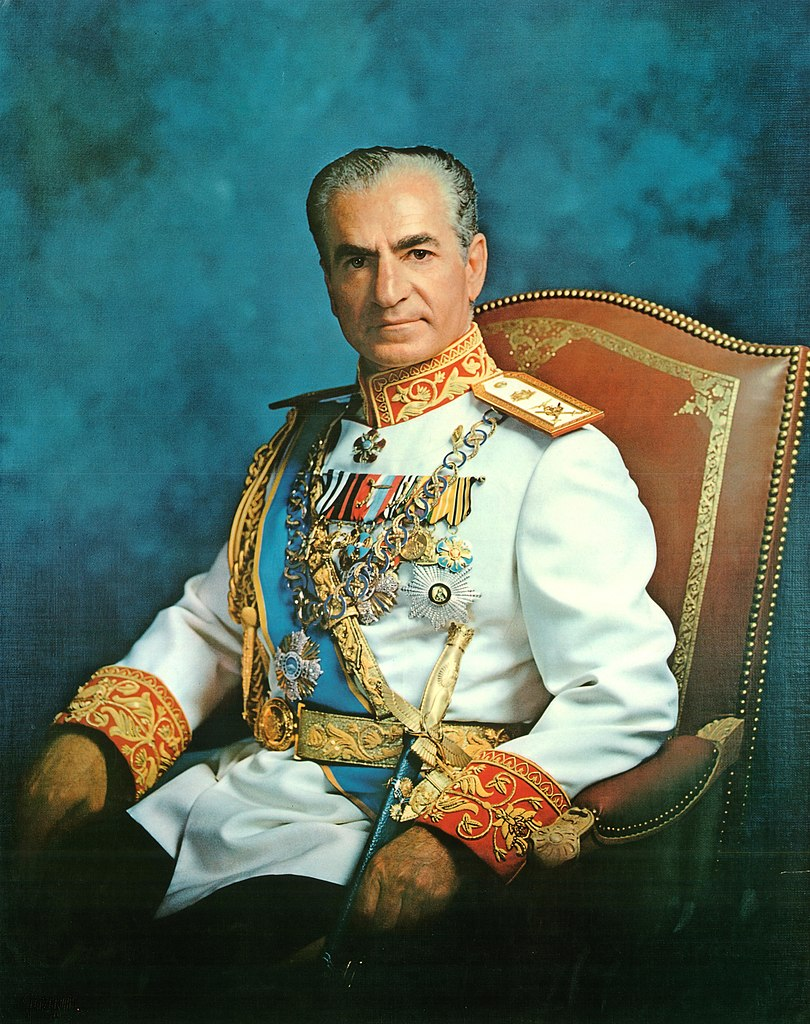
\includegraphics[height=\textheight - 1cm]{shah_of_iran.jpg}}
\end{frame}



\begin{frame}{Banks and maturity transformation}
\justify
Why do we need banks? Banks offer \alert{maturity transformation}.

\justify
Typically savers prefer short-term investments due to liquidity.  Borrowers often need long-term loans. Banks act as intermediaries: they borrow short-term and lend long-term. Think of taking deposits for 1 year and lending 30-years mortgages.

\justify
Banking according to the folklore 3-6-3 rule:
\begin{itemize}
\item Borrow at 3\%.
\item Lend at 6\%.
\item Play golf at 3 p.m.
\end{itemize}
\end{frame}



\begin{frame}{Term risk premium}
\justify
A bank is going to lend some money for 10 years at a fixed interest rate. What factors it should consider when determining the rate of interest for this loan? Should it be 4\% or 10\%?

\begin{itemize}
\justifying
\item Expected average short-term borrowing cost over 10 years.
\item Term risk premium.
\item Expected losses due to the client's default (credit risk).
\item Credit risk premium.
\item Profit margin.
\end{itemize}

\justify
Term risk premium adds a safety buffer in case future borrowing costs will be higher than expected. This is the bank's compensation for holding interest rate risk and performing maturity transformation.
\end{frame}



\begin{frame}{Term risk premium - 2}
\justify
How large is the term risk premium? This variable is unobservable and, probably, time-varying, so we have to estimate it from historical data and models.

\justify
 Adrian-Crump-Moench (ACM) model, US Treasury, 1990--2023:

\begin{tabular}{r|r|r}
2 years & 5 years & 10 years \\ \hline
0.31\% & 0.71\% & 1.16\% 
\end{tabular}

Data: New York Fed.

\justify
Kim-Wright model, US Treasury, 1990--2023:

\begin{tabular}{r|r|r}
2 years & 5 years & 10 years \\ \hline
0.30\% & 0.43\% & 0.77\%
\end{tabular}

Data: St. Louis Fed
\end{frame}



\begin{frame}{Term risk premium - 3}
\center
\begin{tikzpicture}
\begin{axis}[
  width=\textwidth,
  height=\textheight - 1cm,
  date coordinates in=x,
  date ZERO=1960-01-01,
  xtick={1960-01-01, 1970-01-01, 1980-01-01, 1990-01-01, 2000-01-01, 2010-01-01, 2020-01-01},
  xticklabel={\year},
  xmin=1960-01-01,
  xmax=2025-01-01,
  ymin=-2,
  ymax=5,
  grid=major,
  ylabel={\small{ACM 10Y Term Premium, \%}},
  xlabel near ticks,
  ylabel near ticks,
  legend pos=north west,
  %legend style={font=\tiny},
  legend cell align={left}
]
\addplot[color=Set1-A, mark=none, thick] table[x=date, y=acmtp10, col sep=comma]{acm_term_premium.csv};
\draw[thick, color=black] (axis cs: 1960-01-01, 0) -- (axis cs: 2030-01-01, 0);
\end{axis}
\end{tikzpicture}

\scriptsize Data: Federal Reserve Bank of New York.
\end{frame}



\begin{frame}{Borrowing at floating rate}
\justify
Term risk premium is not negligible, especially at times of high uncertainty regarding future inflation and future interest rates. How could we avoid paying the premium (borrow cheaper)?

\justify
We could borrow at floating interest rate which is linked to the bank's short-term funding cost. I.e. shift interest rate risk from the bank to us. On average we will end up paying less interest on our loan.

\justify
How do we measure the short-term funding cost?
\end{frame}



\begin{frame}{London Interbank Offered Rate (LIBOR)}
\justify
In 1969 the Shah of Iran (gentleman on the photo) borrowed \$80mm from a syndicate of London-based banks.

\justify
Members of the syndicate agreed to report their individual short-term borrowing costs. Arithmetic average of the reported rates, rounded to 1/8 of percentage point, would determine the following interest rate payment on the Shah's loan.

\justify
This arithmetic average was called the \alert{London Interbank Offered Rate (LIBOR)}. 
 
\justify
As of 2023 the LIBOR has been discontinued and replaced with other reference interest rates. Nevertheless it paved the way for the market for floating-rate loans and interest rate derivatives.
\end{frame}



\begin{frame}{European Interbank Offered Rate}
\justify
\alert{EURIBOR} is benchmark interest rate for unsecured Euro loans among European bank. It is published by European Money Market Institute (EMMI).

\justify
At which rate a large bank could borrow Euro on the market (from another bank or financial organization)?

\justify
\centering
\begin{tabular}{l|r}
Term (tenor)     & EURIBOR 13.10.2023 \\ \hline
1W (1 week)    & $3.874\%$ \\
1M (1 month)     & $3.860\%$ \\
3M (3 months)    & $3.985\%$ \\
6M (6 months)   & $4.121\%$ \\
12M (12 months) & $4.171\%$ 
\end{tabular}

\justify
*EURIBOR is simple rate (no compounding) in ACT/360 convention.
\end{frame}



\begin{frame}{Computing EURIBOR}
\justify
19 banks from the Eurozone and the UK take part in determining the EURIBOR. Every day each bank submits its interest rate for each of 5 terms (from 1 week to 1 year). The banks follow a methodology which defines 3 "levels":

\justify 
1) Weighted average interest rate of actual transactions which the bank executed on this day on this term. Each transaction should not be smaller than 20mm.

\justify
2) Interpolation of actual transactions from different terms (e.g. interpolate 1M from 1W and 3M) or extrapolating older transactions of the same term.

\justify
3) Interest rates from similar instruments, transactions smaller than 20mm, derivatives, deals with non-financial parties, expert judgment. 

\justify
15\% highest quotes and 15\% lowest quotes are truncated. Arithmetic average of the remaining 70\%, rounded to the third decical digit, is proclaimed the EURIBOR.
\end{frame}



\begin{frame}{Computing EURIBOR - 2}
\centering
\begin{tikzpicture}
		\draw [->,>=triangle 90] (0, 0) -- (9.5, 0);

		\draw [dashed] (0.5,0) node[anchor=north]{$T-1$} .. controls (1.0, 0.5) and (2.5, 0.5) .. (3,0) node[anchor=north]{$T+1$} node[pos=0.5,anchor=south]{spot lag};

		\draw [->,>=triangle 45] (3,0) .. controls (4, 1) and (7, 1) .. (8,0) node[anchor=north]{$T+1+3M$} node[pos=0.5,anchor=south]{$EURIBOR_{T}$};

		\node[anchor=north] at (1.75, 0) {$T$};
		
		\node[circle, fill, inner sep=1.5pt] at (0.5, 0) {};
		\node[circle, fill, inner sep=1.5pt] at (1.75, 0) {};
		\node[circle, fill, inner sep=1.5pt] at (3.0, 0) {};
		\node[circle, fill, inner sep=1.5pt] at (8.0, 0) {};
	\end{tikzpicture}
	
\justify
T--1 (yesterday):  banks were borrowing Euro and gathering data.

T (today): at 11:00 the EMMI announces the average of yesterdays transactions --- 3 months EURIBOR on date $T$.

T+1 (tomorrow): the transactions will be settled (borrowers will receive their Euros).

T+1+3M (in 3 months): the loans will expire (lenders will receive their money back).

\justify
EURIBOR is published on every TARGET2 business day (this is the ECB's payment system). Three months term is computed under "modified following business day"\ convention.
\end{frame}



\begin{frame}{Euro short-term rate}
\justify
\alert{ESTER} is benchmark interest rate for unsecured overnight loans among banks of the Eurozone. It is published by the ECB.

\justify
\centering
\begin{tabular}{l|r}
Term  & ESTER 12.10.2023 \\ \hline
1 day & $3.901\%$
\end{tabular}

\justify
A panel of 48 banks determine ESTER. Each bank informs the ECB about its transactions when it borrows Euro on the market. The ECB discard the lower 25\%  and the 25\% higher values and then computes the weighed average.

\justify
ESTER is simple interest rate (no compounding) in ACT/360 convention.
\end{frame}



\begin{frame}{Computing ESTER}
\justify
\centering
\begin{tikzpicture}
		\draw [->,>=triangle 90] (0, 0) -- (4.0, 0);

		\draw [->, >= triangle 45] (0.5,0) node[anchor=north]{$T$} .. controls (1.0, 0.75) and (2.5, 0.75) .. (3,0) node[anchor=north]{$T+1$} node[pos=0.5,anchor=south]{$ESTER_T$};
\end{tikzpicture}

\justify
T (today): banks borrow Euro overnight and communicate their transactions to the ECB.

T+1 (tomorrow): the ECB announces the weighted average rate --- ESTER for the date T. The loans expire and banks pay Euro back to the lenders.

\justify
Similarly to EURIBOR, ESTER is computed on TARGET2 business days.
\end{frame}



\newcommand{\plotBenchmarkRate}[2] {
	
	\addplot[
		color = #2,
		mark = none,
		thick
	]
	table[
		x=date,
		y=#1,
		col sep=comma
	]
	{euro_benchmark.csv};
}



\begin{frame}{ESTER and EURIBOR}
\centering
\begin{tikzpicture}
\begin{axis}[
  width=\textwidth,
  height=\textheight - 1cm,
  date coordinates in=x,
  date ZERO=2012-01-01,
  xtick={2012-01-01, 2014-01-01, 2016-01-01, 2018-01-01, 2020-01-01, 2022-01-01, 2024-01-01},
  minor xtick={2013-01-01, 2015-01-01, 2017-01-01, 2019-01-01, 2021-01-01, 2023-01-01},
  ytick={-1, 0, 1, 2, 3, 4},
  minor ytick={-0.5, 0.5, 1.5, 2.5, 3.5},
  xticklabel={\year},
  xmin=2012-01-01,
  xmax=2024-01-01,
  ymin=-1,
  ymax=4.5,
  grid=both,
  yticklabel={\pgfmathprintnumber{\tick}\%},
%  ylabel={\small{Курс USDRUB}},
  xlabel near ticks,
  ylabel near ticks,
  legend entries = {
  	   EURIBOR 6M,
      EURIBOR 3M,
      ESTER
  },
  legend cell align={left},
  legend style={at={(0.03,0.97)},anchor=north west}
]

	\plotBenchmarkRate{6m}{Set1-A}
	\plotBenchmarkRate{3m}{Set1-B}
	\plotBenchmarkRate{ester}{Set1-C}
	
	\draw[thick, color=black] (axis cs: 2012-01-01, 0) -- (axis cs: 2024-01-01, 0);
\end{axis}
\end{tikzpicture}

\scriptsize Data: Bundesbank.
\end{frame}



\begin{frame}{EURIBOR futures}
\justify
ICE Futures Europe exchange (former LIFFE) offers three months EURIBOR futures. For examples, \alert{FEIZ3} is December 2023 futures.

\justify
\centering
\begin{tabular}{r|r}
Bid & Offer \\ \hline
95.99 & 96.00
\end{tabular}

\justify
Suppose that we blindly click "buy 10 lots at 96.00".
\begin{itemize}
\justifying
\item No initial cost to be paid today.
\item On December 18 2023** the exchange will set final price for the futures at $F = 100 - X$, where 
$X$ is the EURIOBOR which will be announced on that day.
\item We will earn $10 \cdot (F - 96.00) \cdot \EUR{2\,500}$, where \EUR{2\,500} is a constant from the futures' specification.
\end{itemize}

\justify
*FEI is contract code. Z is month code (H for March, M for June, U for September, Z for December). 3 is last digit of the year.

\justify
**Two business days prior to the third Wednesday of the month.
\end{frame}



\begin{frame}{EURIBOR futures - 2}
\justify
I know in advance that in December I will become richer by \EUR{1\,000\,000}. I plan to deposit the money for three months, collect it in March and go on holiday. I face \alert{interest rate risk}: I do not know how  much money I will have by March.
\justify
Solution: buy one lot of EURIBOR December futures at 96.00.

\justify
Suppose that by December 18 the EURIBOR will drop to $3.50\%$.
\begin{itemize}
\justifying
\item The exchange will set final price at $100 - 3.50 = 96.50$.
\item Gain on the futures is $(96.50-96.00)\cdot\EUR{2\,500} = \EUR{1\,250}$.
\item Three months deposit at EURIBOR $3.50\%$ will earn

$\EUR{1\,000\,000} \cdot 0.035 / 4 = \EUR{8\,750}$.
\item In total, I will earn $\EUR{1\,250} + \EUR{8\,750} = \EUR{10\,000}$.
\end{itemize} 

\justify
I would have earned the same amount if EURIBOR was $4.00\%$:

$\EUR{1\,000\,000} \cdot 0.04/4 =\EUR{10\,000}$.
\end{frame}



\begin{frame}{EURIBOR futures - 3}
\justify
We bought the December futures in October at 96.00. In December we deposited cash at the prevailing EURIBOR. How much money are we going to make?\
\justify
\centering
\begin{tabular}{r|r|r|r|r}
EURIBOR   & Final price & Futures         & Deposit & Total \\ \hline
$2.50\%$ & 97.50        & $\EUR{3\,750}$      &   $\EUR{6\,250}$  & $\EUR{10\,000}$ \\
$3.00\%$ & 97.00        & $\EUR{2\,500}$      &   $\EUR{7\,500}$  & $\EUR{10\,000}$ \\
$3.50\%$ & 96.50        & $\EUR{1\,250}$      & $\EUR{8\,750}$  & $\EUR{10\,000}$ \\
$4.00\%$ & 96.00        & $\EUR{0}$                & $\EUR{10\,000}$  & $\EUR{10\,000}$ \\
$4.50\%$ & 95.50        & $-\EUR{1\,250}$    & $\EUR{11\,250}$ & $\EUR{10\,000}$ \\
$5.00\%$ & 95.00        & $-\EUR{2\,500}$    & $\EUR{12\,500}$ & $\EUR{10\,000}$
\end{tabular}

\justify
When we buy 1 futures lot at $100-X$ we secure interest rate for a future deposit of \EUR{1\,000\,000} at EURIBOR. When we sell we secure a future loan of \EUR{1\,000\,000} at EURIBOR.
\end{frame}



\begin{frame}{Interest rate swap}
\justify
\alert{Interest rate swap} is a derivative in which two parties exchange interest payments at a fixed rate and a floating (reference) rate.

\justify
Parameters of a swap:
\begin{itemize}
\justifying
\item Term or maturity. For example, 1 year.
\item Notional amount or principal amount --- an amount that accrues interest. For example, \EUR{1} million.
\item Coupon or swap rate --- fixed interest rate which is paid by one f the parties. For example, $3.0\%$ per annum.
\item Reference rate --- particular interest rate benchmark which is paid by the other party. For example, 3M EURIBOR.
\end{itemize}

\justify
Buying a swap means receiving the floating rate and paying the fixed rate. Selling a swap means paying the floating rate and receiving the fixed rate..
\end{frame}



\begin{frame}{Interest rate swap - 2}
\centering
\begin{tikzpicture}[thick, scale=0.75]
		\draw (0, 0) node[rectangle,draw,rounded corners,anchor=south,minimum height=1cm] {Company A} -- (0, -7);
		\draw (9.5, 0) node[rectangle,draw,rounded corners,anchor=south,minimum height=1cm] {Company B} -- (9.5, -7);

		\draw [dashed,->,>=triangle 90] (0, -1) node[label=left:{$T_0$}]{} -- (4.5, -1) node[pos=0.5,anchor=south]{$\EUR{1\,000\,000}$};

		\draw [dashed,->,>=triangle 90] (9.5, -1) node[label=right:{\text{$E_1$ fixing}}]{} -- (5, -1) node[pos=0.5,anchor=south]{\euro 1\,000\,000};

		\draw [->,>=triangle 90] (0, -2.5) node[label=left:{$T_1 = \text{3M}$}]{} -- (4.5, -2.5) node[pos=0.5,anchor=south]{$\EUR{1\,000\,000} \cdot \dfrac{3.0\%}{4}$};

		\draw [snake=snake,->,>=triangle 90] (9.5, -2.5)  node[label=right:{\text{$E_2$ fixing}}]{} -- (5, -2.5) node[pos=0.5,anchor=south] {$\EUR{1\,000\,000} \cdot \dfrac{E_1}{4}$};

		\draw [->,>=triangle 90] (0, -4) node[label=left:{$T_2 = \text{6M}$}]{} -- (4.5, -4) node[pos=0.5,anchor=south]{$\EUR{1\,000\,000} \cdot \dfrac{3.0\%}{4}$};

		\draw [snake=snake,->,>=triangle 90] (9.5, -4)  node[label=right:{\text{$E_3$ fixing}}]{} -- (5, -4) node[pos=0.5,anchor=south] {$\EUR{1\,000\,000} \cdot \dfrac{E_2}{4}$};

		\draw [->,>=triangle 90] (0, -5.5) node[label=left:{$T_3 = \text{9M}$}]{} -- (4.5, -5.5) node[pos=0.5,anchor=south]{$\EUR{1\,000\,000} \cdot \dfrac{3.0\%}{4}$};

		\draw [snake=snake,->,>=triangle 90] (9.5, -5.5)  node[label=right:{\text{$E_4$} fixing}]{} -- (5, -5.5) node[pos=0.5,anchor=south] {$\EUR{1\,000\,000} \cdot \dfrac{E_3}{4}$};
		\draw [->,>=triangle 90] (0, -7) node[label=left:{$T_4 = \text{12M}$}]{} -- (4.5, -7) node[pos=0.5,anchor=south]{$\EUR{1\,000\,000} \cdot \dfrac{3.0\%}{4}$};

		\draw [snake=snake,->,>=triangle 90] (9.5, -7) -- (5, -7) node[pos=0.5,anchor=south] {$\EUR{1\,000\,000} \cdot \dfrac{E_4}{4}$};
\end{tikzpicture}
\end{frame}



\begin{frame}{Managing interest rate risk}
\justify
An interest rate swap turns a loan at floating rate (for example EURIBOR+1\%) into a loan at fixed rate (for example, 4.0\%), and vice versa..

\justify
\centering
	\begin{tikzpicture}[thick]

		\tikzstyle{company}=[rectangle,draw,rounded corners,minimum height=1.2cm,minimum width=3cm];
		\tikzstyle{fixed}=[->,>=triangle 90];
		\tikzstyle{floating}=[snake=snake,->,>=triangle 90];

		\node (A) at (0, 0) [company] {Company A};
		\node (B) at (7, 0) [company] {Company B};
		\node (Deutsche) at (0, -3) [company] {Deutsche};
		\node (Citi) at (7, -3) [company] {Citi};

		\draw [fixed] ([yshift=0.2cm]A.east) -- ([yshift=0.2cm]B.west) node[pos=0.5,anchor=south]{3.0\%};

		\draw [floating] ([yshift=-0.2cm]B.west) -- ([yshift=-0.2cm]A.east) node[pos=0.5,anchor=north]{EURIBOR};

		\draw [floating] (A.south) -- (Deutsche.north) node[pos=0.5,anchor=west]{EURIBOR + 1\%};

		\draw [fixed] (B.south) -- (Citi.north) node[pos=0.5,anchor=east]{$3.5\%$};
	\end{tikzpicture}

\justify
Company A pays 4.0\%, company B pays EURIBOR + 0.5\%.
\end{frame}



%\begin{frame}{Loans at floating rate}
%\justify
%Suppose that we are a small company with low credit rating. We need a loan for 5 years.
%
%\begin{itemize}
%\justifying
%\item It costs EURIBOR + 2\% to borrow the money for 3 months. 
%\item It costs 7.0\% to borrow them money for 5 years from a bank.
%\item 5 years swap rate is 4.0\%.
%\end{itemize}
%
%\justify
%We can make a bet we will be able to borrow at EURIBOR+2\% in the future just like today. Then we can start a chain of 3 months loans (we borrow at time $T$ to repay the debt which we borrowed at time $T-1$). Then buy a swap to hedge interest rate risk.
%
%\begin{itemize}
%\justifying
%\item Loans: pay EURIBOR+2\%.
%\item Bought swap: pay 4\%, receive EURIBOR.
%\item Net: pay 6\%.
%\end{itemize}
%
%\justify
%Is there a catch? Our credit quality may deteriorate in future. One day we may have to renew the loan at EURIBOR+10\% and the strategy will blow up.
%\end{frame}



\begin{frame}{Present value}
\justify
\alert{Present value} of a cashflow of $N$ units of currency in $T$ years is the price which market participants would be willing to pay today to be entitled for this future cashflow.

\justify
How much USD you would be willing to pay today (present value, PV) to be entitled to receive 1\,050\,000 USD in one year (future value, FV)? Suppose that the market offers and ideal risk-free deposit at 5\% (no interest compounding).

\begin{align*}
PV = \frac{FV}{1+rT} = \frac{1\,050\,000}{1 + 5\%} = 1\,000\,000
\end{align*}

\justify
Nobody will be willing to pay more than 1\,000\,000 current dollars for 1\,050\,000 future dollars. It would be more profitable to deposit current dollars at 5\%.

\justify
There is no sense in selling 1\,050\,000 future dollars cheaper than 1\,000\,000 today, because one could borrow dollars today at 5\% and pay the debt in 1 year.
\end{frame}



\begin{frame}{Discount factor}
\justify
\alert{Discount factor} for a future date $T$ is present value of a cashflow of 1 unit of a currency on date $T$. How many units of a currency you need to posses today in order to turn it into 1 unit of a currency by time $T$?

\justify
The answer depends on risk-free interest rate:
\begin{align*}
\delta_T = \frac{1}{1 + rT} \quad \text{(simple interest)}
\end{align*}

\justify
For example, suppose that risk-free interest rate is 5\%.  Discount factor for 1 year is then
\begin{align*}
\delta_1 = \frac{1}{1.05} \approx 0.9524
\end{align*}
\end{frame}



\begin{frame}{Fair swap rate}
\centering
\begin{tikzpicture}[thick, scale=0.7]
		\draw (0, 0) node[rectangle,draw,rounded corners,anchor=south,minimum height=1cm] {Company A} -- (0, -3);
		\draw (7.5, 0) node[rectangle,draw,rounded corners,anchor=south,minimum height=1cm] {Company B} -- (7.5, -3);

		\draw [->,>=triangle 90] (0, -1) node[label=left:{$T_1$}]{} -- (3.5, -1) node[pos=0.5,anchor=south]{$N \cdot x \cdot t_1$};

		\draw [snake=snake,->,>=triangle 90] (7.5, -1)  -- (4, -1) node[pos=0.5,anchor=south] {$N \cdot E_1 \cdot t_1$};
		
		\draw [->,>=triangle 90] (0, -2.5) node[label=left:{$T_2$}]{} -- (3.5, -2.5) node[pos=0.5,anchor=south]{$N \cdot x \cdot t_2$};

		\draw [snake=snake,->,>=triangle 90] (7.5, -2.5) -- (4, -2.5) node[pos=0.5,anchor=south] {$N \cdot E_2 \cdot t_2$};

		\draw (0, -3.5) -- (0, -4.5);				
		\draw (7.5, -3.5) -- (7.5, -4.5);

		\draw [->,>=triangle 90] (0, -4) node[label=left:{$T_i$}]{} -- (3.5, -4) node[pos=0.5,anchor=south]{$N \cdot x \cdot t_i$};

		\draw [snake=snake,->,>=triangle 90] (7.5, -4) -- (4, -4) node[pos=0.5,anchor=south] {$N \cdot E_i \cdot t_i$};
\end{tikzpicture}

\justify
$N$ --- notional amount.

$T_i$ --- number of years till the $i$-th payment.

$E_i$ --- expected EURIBOR on date $T_{i-1}$.

$t_i = T_i - T_{i-1}$ --- year fractions for interest accrual.

$\delta_i$ --- discount factor from date $T_i$ to today.

\justify
What should be fair swap rate (fair coupon) $x$?
\end{frame}



\begin{frame}{Fair swap rate - 2}
\justify
Present values of company A's payments and company B's payments should match. Otherwise one of the parties is just giving the money away.

\justify
\begin{align*}
\sum\limits_{i=1}^{n} N \cdot x \cdot t_i \cdot \delta_i 
= \sum\limits_{i=1}^{n} N \cdot E_i \cdot t_i \cdot \delta_i
\end{align*}
\begin{align*}
x = \frac{\sum\limits_{i=1}^{n} E_i t_i \delta_i}{\sum\limits_{i=1}^{n} t_i \delta_i}
\end{align*}

\justify
If someone tells us future values of the EURIBOR $E_i$ and discount factors $\delta_i$ we will be able to compute fair coupon for any interest rate swap.
\end{frame}



\begin{frame}{Fair swap rate - 3}
\justify
Suppose that the discount rate is close to zero, and all discount factors are close to zero. $\delta_i \approx1$.

\justify
Lets ignore peculiarities of the Gregorian calendar and assume that all intervals between interest rate payments are equal. For example, $t_i = t = 1/4$ in a swap with quarterly payments.

\begin{align*}
x = \frac{\sum\limits_{i=1}^{n} E_i t_i \delta_i}{\sum\limits_{i=1}^{n} t_i \delta_i}
\approx
\frac{\sum\limits_{i=1}^{n} E_i t}{\sum\limits_{i=1}^{n} t}
=
\frac{\sum\limits_{i=1}^{n} E_i}{n}
\end{align*}

\justify
Captain Obvious is reporting: swap rate is average of EURIBORs during the swap's lifetime.
\end{frame}



\begin{frame}{Computing expected EURIBOR values}
\justify
Bloomberg and Reuters terminals broadcast the following quotes from the market for three months EURIBOR swaps. This is our observable reality.

\justify
\centering
\begin{tabular}{l|r}
Instrument        & Swap rate (coupon) \\ \hline
Last fixing & 3.00\% \\
6M swap           & 3.40\% \\
9M swap           & 3.60\% \\
1Y swap           & 3.70\% \\
18M swap          & 3.75\% \\
2Y swap           & 3.60\%
\end{tabular}

\end{frame}



\begin{frame}{Computing expected EURIBOR values - 2}
\centering
\begin{tikzpicture}[thick, scale=0.7]
		\draw (0, 0) node[rectangle,draw,rounded corners,anchor=south,minimum height=1cm] {Company A} -- (0, -2.5);
		\draw (7.5, 0) node[rectangle,draw,rounded corners,anchor=south,minimum height=1cm] {Company B} -- (7.5, -2.5);

		\draw [->,>=triangle 90] (0, -1) node[label=left:{3M}]{} -- (3.5, -1) node[pos=0.5,anchor=south]{$3.40\%$};

		\draw [snake=snake,->,>=triangle 90] (7.5, -1)  -- (4, -1) node[pos=0.5,anchor=south] {$3.00\%$};
		
		\draw [->,>=triangle 90] (0, -2.5) node[label=left:{6M}]{} -- (3.5, -2.5) node[pos=0.5,anchor=south]{$3.40\%$};

		\draw [snake=snake,->,>=triangle 90] (7.5, -2.5) -- (4, -2.5) node[pos=0.5,anchor=south] {$E_2$};
\end{tikzpicture}

\justify
We know 6 months swap rate ($3.40\%$). We also know the most recent EURIBOR fxing ($3.00\%$) which defines the very first floating payment. We can derive "implied"\ value of $E_2$.
\begin{align*}
3.40\% + 3.40\% &= 3.00\% + E_2 \Rightarrow \\
E_2 &= 3.80\%
\end{align*}

\end{frame}



\begin{frame}{Musings on "implied"\ values}
\justify
Can we hope that the implied value $E_2=3.80\%$ is correct? No, we cannot. Most probably, the prevailing EURIBOR in three months will be different. On average, interest rates tend to be lower than "implied"\ rates which one could derive from the market swap rates.

\justify
Implied interest rate is just a rate that corresponds to current market swap rates. These are two equivalent views on the same reality:

\justify
1) The latest fixing is $3.00\%$, 6 months swap rate is $3.40\%$.

\justify
2) The latest fixing is $3.00\%$, EURIBOR in 3 months is $3.80\%$.
\end{frame}



\begin{frame}{Musings on "implied"\ values - 2}
\justify
It does not matter whether the market is correct when it estimates the future value of $E_2$. It is important that the market offers liquid instruments which allow us hedge interest rate risk.

\justify
Suppose we will have to pay interest of $E_2$ on  a floating-rate loan. Then lets buy a 6 months swap.

\centering
\begin{tabular}{l|r|r|r}
    & \multicolumn{2}{c|}{Swap} & Loan \\ \hline
Today &          0  &  0            & 0 \\
3M      & $-3.40\%$  &  $+3.00\%$   & 0 \\
6M      & $-3.40\%$  &  $+E_2$       & $-E_2$ \\ \hline
PV       & \multicolumn{3}{c}{-3.80\%}
\end{tabular}

\justify
With a swap we can eliminate all the uncertainty and live in a world where the future EURIBOR $E_2$ is always 3.80\%.
\end{frame}



\begin{frame}{Computing expected EURIBOR values - 3}
\centering
\begin{tikzpicture}[thick, scale=0.7]
		\draw (0, 0) node[rectangle,draw,rounded corners,anchor=south,minimum height=1cm] {Company A} -- (0, -4);
		\draw (7.5, 0) node[rectangle,draw,rounded corners,anchor=south,minimum height=1cm] {Company B} -- (7.5, -4);

		\draw [->,>=triangle 90] (0, -1) node[label=left:{3M}]{} -- (3.5, -1) node[pos=0.5,anchor=south]{$3.60\%$};

		\draw [snake=snake,->,>=triangle 90] (7.5, -1)  -- (4, -1) node[pos=0.5,anchor=south] {$3.00\%$};
		
		\draw [->,>=triangle 90] (0, -2.5) node[label=left:{6M}]{} -- (3.5, -2.5) node[pos=0.5,anchor=south]{$3.60\%$};

		\draw [snake=snake,->,>=triangle 90] (7.5, -2.5) -- (4, -2.5) node[pos=0.5,anchor=south] {$3.80\%$};
		
		\draw [->,>=triangle 90] (0, -4) node[label=left:{9M}]{} -- (3.5, -4) node[pos=0.5,anchor=south]{$3.60\%$};

		\draw [snake=snake,->,>=triangle 90] (7.5, -4) -- (4, -4) node[pos=0.5,anchor=south] {$E_3$};
\end{tikzpicture}

\justify
We know 9 months swap rate (3.60\%) and the first two EURIBORs (3.00\% и 3.80\%). We can compute implied value of $E_3$.
\begin{align*}
3.60\% + 3.60\% + 3.60\% &= 3.0\% + 3.80\% + E_3 \Rightarrow \\
E_3 &= 4.00\%
\end{align*}
\end{frame}



\begin{frame}{Computing expected EURIBOR values - 4}
\centering
\begin{tikzpicture}[thick, scale=0.7]
		\draw (0, 0) node[rectangle,draw,rounded corners,anchor=south,minimum height=1cm] {Company A} -- (0, -5.5);
		\draw (7.5, 0) node[rectangle,draw,rounded corners,anchor=south,minimum height=1cm] {Company B} -- (7.5, -5.5);

		\draw [->,>=triangle 90] (0, -1) node[label=left:{3M}]{} -- (3.5, -1) node[pos=0.5,anchor=south]{$3.70\%$};

		\draw [snake=snake,->,>=triangle 90] (7.5, -1)  -- (4, -1) node[pos=0.5,anchor=south] {$3.00\%$};
		
		\draw [->,>=triangle 90] (0, -2.5) node[label=left:{6M}]{} -- (3.5, -2.5) node[pos=0.5,anchor=south]{$3.70\%$};

		\draw [snake=snake,->,>=triangle 90] (7.5, -2.5) -- (4, -2.5) node[pos=0.5,anchor=south] {$3.80\%$};
		
		\draw [->,>=triangle 90] (0, -4) node[label=left:{9M}]{} -- (3.5, -4) node[pos=0.5,anchor=south]{$3.70\%$};

		\draw [snake=snake,->,>=triangle 90] (7.5, -4) -- (4, -4) node[pos=0.5,anchor=south] {$4.00\%$};
		
		\draw [->,>=triangle 90] (0, -5.5) node[label=left:{12M}]{} -- (3.5, -5.5) node[pos=0.5,anchor=south]{$3.70\%$};

		\draw [snake=snake,->,>=triangle 90] (7.5, -5.5) -- (4, -5.5) node[pos=0.5,anchor=south] {$E_4$};
\end{tikzpicture}

\justify
We know 12 months swap rate (3.70\%) and the first three EURIBORs (3.00\%, 3.80\% и 4.00\%). We can compute implied value of $E_4$.
\begin{align*}
3.70\%+3.70\%+3.70\%+3.70\% &= 3.00\% + 3.80\% + 4.00\% + E_4 \Rightarrow \\
E_4 &= 4.00\%
\end{align*}
\end{frame}



\begin{frame}{Computing expected EURIBOR values - 5}
\centering
\begin{tikzpicture}[thick, scale=0.7]
		\draw (0, 0) node[rectangle,draw,rounded corners,anchor=south,minimum height=1cm] {Company A} -- (0, -8.5);
		\draw (7.5, 0) node[rectangle,draw,rounded corners,anchor=south,minimum height=1cm] {Company B} -- (7.5, -8.5);

		\draw [->,>=triangle 90] (0, -1) node[label=left:{3M}]{} -- (3.5, -1) node[pos=0.5,anchor=south]{$3.75\%$};

		\draw [snake=snake,->,>=triangle 90] (7.5, -1)  -- (4, -1) node[pos=0.5,anchor=south] {$3.00\%$};
		
		\draw [->,>=triangle 90] (0, -2.5) node[label=left:{6M}]{} -- (3.5, -2.5) node[pos=0.5,anchor=south]{$3.75\%$};

		\draw [snake=snake,->,>=triangle 90] (7.5, -2.5) -- (4, -2.5) node[pos=0.5,anchor=south] {$3.80\%$};
		
		\draw [->,>=triangle 90] (0, -4) node[label=left:{9M}]{} -- (3.5, -4) node[pos=0.5,anchor=south]{$3.75\%$};

		\draw [snake=snake,->,>=triangle 90] (7.5, -4) -- (4, -4) node[pos=0.5,anchor=south] {$4.00\%$};
		
		\draw [->,>=triangle 90] (0, -5.5) node[label=left:{12M}]{} -- (3.5, -5.5) node[pos=0.5,anchor=south]{$3.75\%$};

		\draw [snake=snake,->,>=triangle 90] (7.5, -5.5) -- (4, -5.5) node[pos=0.5,anchor=south] {$4.00\%$};
		
				\draw [->,>=triangle 90] (0, -7) node[label=left:{15M}]{} -- (3.5, -7) node[pos=0.5,anchor=south]{$3.75\%$};

		\draw [snake=snake,->,>=triangle 90] (7.5, -7) -- (4, -7) node[pos=0.5,anchor=south] {$E_5$};
		
				\draw [->,>=triangle 90] (0, -8.5) node[label=left:{18M}]{} -- (3.5, -8.5) node[pos=0.5,anchor=south]{$3.75\%$};

		\draw [snake=snake,->,>=triangle 90] (7.5, -8.5) -- (4, -8.5) node[pos=0.5,anchor=south] {$E_6$};
\end{tikzpicture}
\end{frame}



\begin{frame}{Computing expected EURIBOR values - 6}
\justify
There is no observable quote for a 15 months swap, we only have 18 months swap rate. This leaves us with single equation and two unknown EURIBORs $E_5$ и $E_6$.
\begin{align*}
3.00\%+3.80\%+4.00\%+4.00\%+E_5+E_6 = 6\cdot3.75\%
\end{align*}

\justify
Suppose that there is linear dependence between interest rates. $E_5$ is higher than $E_4$ by the same amount as $E_6$ is higher than $E_5$.
\begin{align*}
\begin{cases}
3.00\%+3.80\%+4.00\%+4.00\%+E_5+E_6 = 6\cdot3.75\% \\
E_5 - 4.00\% = E_6 - E_5
\end{cases}
\end{align*}

Therefore, if we assume linear interpolation, we can compute
\begin{align*}
\begin{cases}
E_5 = 3.90\% \\
E_6 = 3.80\%
\end{cases}
\end{align*}
\end{frame}



\begin{frame}{Adding discount factors}
\centering
\begin{tikzpicture}[thick, scale=0.7]
		\draw (0, 0) node[rectangle,draw,rounded corners,anchor=south,minimum height=1cm] {Company A} -- (0, -2.5);
		\draw (7.5, 0) node[rectangle,draw,rounded corners,anchor=south,minimum height=1cm] {Company B} -- (7.5, -2.5);

		\draw [->,>=triangle 90] (0, -1) node[label=left:{3M}]{} -- (3.5, -1) node[pos=0.5,anchor=south]{$S_{6M}t_1\alert{\delta_1}$};

		\draw [snake=snake,->,>=triangle 90] (7.5, -1)  -- (4, -1) node[pos=0.5,anchor=south] {$E_1t_1\alert{\delta_1}$};
		
		\draw [->,>=triangle 90] (0, -2.5) node[label=left:{6M}]{} -- (3.5, -2.5) node[pos=0.5,anchor=south]{$S_{6M}t_2\alert{\delta_2}$};

		\draw [snake=snake,->,>=triangle 90] (7.5, -2.5) -- (4, -2.5) node[pos=0.5,anchor=south] {$\alert{E_2}t_2\alert{\delta_2}$};
\end{tikzpicture}

\justify
Lets get back to reality and include discounting into our model. We need discount factors for 3 months and 6 months,
$\delta_1$ и $\delta_2$. Usually we do not know then beforehand, so we end up with a single equation and three unknown variables. 
\begin{align*}
S_{6M}t_1\alert{\delta_1} + S_{6M}t_2\alert{\delta_2} = E_1t_1\delta_1 + \alert{E_2}t_2\alert{\delta_2}
\end{align*}

\justify
What shall we do?
\end{frame}



\begin{frame}{Risk-free investment at EURIBOR}
\justify
Suppose that the three-month EURIBOR interest rate is risk-free. This is reasonable assumption, because usually we hear concerns about a bank's creditworthiness in advance.

\justify
We can construct a chain of risk-free deposits at EURIBOR

1) Pick a solid bank and deposit our money at the current EURIBOR.

2) Wait for three months

3) Collect the money and return to step 1..

\justify
\centering
\begin{tikzpicture}
		\draw [->,>=triangle 90] (0.5, 0) -- (11, 0);

		\draw [->,>=triangle 45] (0.5,0) node[anchor=north east]{0} .. controls (1, 0.5) and (2, 0.5) .. (2.5,0) node[anchor=north]{$T_1$} node[pos=0.5,anchor=south]{$E_1$};

		\draw [->,>=triangle 45] (2.5,0) .. controls (3, 0.5) and (4, 0.5) .. (4.5,0) node[anchor=north]{$T_2$} node[pos=0.5,anchor=south]{$E_2$};

		\draw [->,>=triangle 45] (4.5,0) .. controls (5, 0.5) and (6, 0.5) .. (6.5,0) node[anchor=north]{$T_3$} node[pos=0.5,anchor=south]{$E_3$};
		
		\draw [dashed] (6.5,0) .. controls (7, 0.5) and (8, 0.5) .. (8.5,0);
		
		\draw [->,>=triangle 45] (8.5,0) node[anchor=north]{$T_{n-1}$} .. controls (9, 0.5) and (10, 0.5) .. (10.5,0) node[anchor=north]{$T_n$} node[pos=0.5,anchor=south]{$E_n$};
	\end{tikzpicture}
%\justify
%Каждый раз на шаге 1 мы можем (но не обязаны) выбирать новый банк, если кредитный рейтинг предыдущего банка нам больше не нравится.
\end{frame}



\begin{frame}{Risk-free investment at EURIBOR - 2}
\centering
\begin{tikzpicture}
		\draw [->,>=triangle 90] (0.5, 0) -- (11, 0);

		\draw [->,>=triangle 45] (0.5,0) node[anchor=north]{$T_0$} .. controls (1, 0.5) and (2, 0.5) .. (2.5,0) node[anchor=north]{$T_1$} node[pos=0.5,anchor=south]{$E_1$};

		\draw [->,>=triangle 45] (2.5,0) .. controls (3, 0.5) and (4, 0.5) .. (4.5,0) node[anchor=north]{$T_2$} node[pos=0.5,anchor=south]{$E_2$};

		\draw [->,>=triangle 45] (4.5,0) .. controls (5, 0.5) and (6, 0.5) .. (6.5,0) node[anchor=north]{$T_3$} node[pos=0.5,anchor=south]{$E_3$};
		
		\draw [dashed] (6.5,0) .. controls (7, 0.5) and (8, 0.5) .. (8.5,0);
		
		\draw [->,>=triangle 45] (8.5,0) node[anchor=north]{$T_{n-1}$} .. controls (9, 0.5) and (10, 0.5) .. (10.5,0) node[anchor=north]{$T_n$} node[pos=0.5,anchor=south]{$E_n$};
		
		\node [anchor=north] at (1.5, 0) {$t_1$};
		\node [anchor=north] at (3.5, 0) {$t_2$};
		\node [anchor=north] at (5.5, 0) {$t_3$};
		\node [anchor=north] at (9.5, 0) {$t_n$};
	\end{tikzpicture}
	
\justify
We invested $N_0$ euro into a chain of deposits. How many Euros we will accumulate by the time $T_n$?
\begin{align*}
N_n = N_0(1 + E_1t_1)(1 + E_2t_2) ... (1 + E_nt_n)
\end{align*}

\justify
What is the discount factor for the terminal date of the chain $T_n$?
\begin{align*}
\delta_n = \frac{1}{(1 + E_1t_1)(1 + E_2t_2) ... (1 + E_nt_n)}
\end{align*}
\end{frame}



\begin{frame}{Adding discount factors - 2}
\centering
\begin{tikzpicture}[thick, scale=0.7]
		\draw (0, 0) node[rectangle,draw,rounded corners,anchor=south,minimum height=1cm] {Company A} -- (0, -2.5);
		\draw (7.5, 0) node[rectangle,draw,rounded corners,anchor=south,minimum height=1cm] {Company B} -- (7.5, -2.5);

		\draw [->,>=triangle 90] (0, -1) node[label=left:{3M}]{} -- (3.5, -1) node[pos=0.5,anchor=south]{$S_{6M}t_1\alert{\delta_1}$};

		\draw [snake=snake,->,>=triangle 90] (7.5, -1)  -- (4, -1) node[pos=0.5,anchor=south] {$E_1t_1\alert{\delta_1}$};
		
		\draw [->,>=triangle 90] (0, -2.5) node[label=left:{6M}]{} -- (3.5, -2.5) node[pos=0.5,anchor=south]{$S_{6M}t_2\alert{\delta_2}$};

		\draw [snake=snake,->,>=triangle 90] (7.5, -2.5) -- (4, -2.5) node[pos=0.5,anchor=south] {$\alert{E_2}t_2\alert{\delta_2}$};
\end{tikzpicture}

\justify
We have just established a link between future EURIBOR values $E_i$ and discount factors $\delta_i$. Now we have a system of three variables and three equations.
\begin{align*}
\begin{cases}
S_{6M}t_1\alert{\delta_1} + S_{6M}t_2\alert{\delta_2} = E_1t_1\delta_1 + \alert{E_2}t_2\alert{\delta_2} \\
\alert{\delta_1} = \dfrac{1}{1+E_1t_1} \\
\alert{\delta_2} = \dfrac{1}{(1+E_1t_1)(1+\alert{E_2}t_2)}
\end{cases}
\Rightarrow E_2 \approx 3.804\%
\end{align*}
\end{frame}



\begin{frame}{Bootstrapping the yield curve}
\justify
If we consider EURIBOR a risk-free rate, it is convenient to represent the future values as a set of discount factors $\delta_i$. 

\justify
Future EURIBOR value for a deposit which will begin in $T_1$ years and will end in $T_2 = T_1 + 0.25$ years is
\begin{align*}
E(T_1, T_2) = \frac{\dfrac{\delta_{T_1}}{\delta_{T_2}} - 1}{T_2 - T_1}
\end{align*}

\justify
The step-by-step algorithm to compute discount factors and future interest rates from market swap rates is called the \alert{bootstrap} method. A few financial mathematics libraries, such as QuantLib and tf-quant-finance, implement this method.
\end{frame}



\begin{frame}{Bootstrapping the yield curve: an example}
\justify
Consider the following market quotes (swap rates) for interest rate swaps referencing the three-months EURIBOR: 

\justify
\centering
\begin{tabular}{l|r|l|r}
Maturity & Swap rate & Maturity & Swap rate \\ \hline
3m   & 3.00\% & 4y   & 3.25\% \\
6m   & 3.40\% & 5y   & 3.15\% \\
9m   & 3.60\% & 6y   & 3.10\% \\
1y   & 3.70\% & 7y   & 3.05\% \\
18m  & 3.75\% & 8y   & 3.00\% \\
2y   & 3.60\% & 9y   & 3.00\% \\
3y   & 3.40\% & 10y  & 3.00\% 
\end{tabular}
\end{frame}



\begin{frame}{Interpolation: an example}
\begin{tikzpicture}
\begin{axis}[
  width=\textwidth,
  height=\textheight - 1cm,
  date coordinates in=x,
  date ZERO=2012-01-01,
  xtick={2023-01-01, 2024-01-01, 2025-01-01, 2026-01-01, 2027-01-01, 2028-01-01, 2029-01-01, 2030-01-01},
  %minor xtick={2013-01-01, 2015-01-01, 2017-01-01, 2019-01-01, 2021-01-01},
  %ytick={-0.5, 0, 0.5, 1.0, 1.5},
  %minor ytick={-0.75, -0.25, 0.25, 0.75, 1.25},
  xticklabel={\year},
  xmin=2023-03-13,
  xmax=2030-01-01,
  %ymin=-0.75,
  %ymax=1.5,
  grid=major,
  ylabel={\small{EURIBOR, basis points}},
  xlabel near ticks,
  ylabel near ticks,
  legend entries = {	
  	   Linear,
  	   Spline
  },
  legend cell align={left},
  legend pos = north east
]

	\addplot[
		color = Set1-A,
		mark = none,
		very thick
	]
	table[
		x=date,
		y=linear,
		col sep=comma
	]
	{euribor_bootstrap.csv};
	
	\addplot[
		color = Set1-B,
		mark = none,
		very thick
	]
	table[
		x=date,
		y=spline,
		col sep=comma
	]
	{euribor_bootstrap.csv};
	
	\draw[thick, color=black] (axis cs: 2012-01-01, 0) -- (axis cs: 2030-01-01, 0);
\end{axis}
\end{tikzpicture}
\end{frame}



\begin{frame}{Forward-forward swap}
\justify
Consider a non-standard ("forward-forward") interest rate swap which will begin in 2.5 years from now and will end in 5 years from now ("30M x 5Y").

\justify
We know future EURIBOR values and discount factors, so we can pick a swap rate which makes the swap have zero initial present value.

\justify
\centering
\begin{tabular}{l|l|l}
& Receive & Pay \\ \hline
Effective date & 15.09.2025 & 15.09.2025 \\ 
Maturity date  & 15.03.2028 & 15.03.2028 \\
Notional       & \EUR{1\,000\,000} & \EUR{1\,000\,000} \\
Frquency       & Semi-annually     & Quarterly \\
Rate           & \alert{2.7646\%}          & EURIBOR-3M   \\
Basis          & ACT/360           & ACT/360
\end{tabular}
\end{frame}



\begin{frame}{Market risk: an example}
\justify
PV01 (present value of 1 bp) or DV01 (dollar value of 1 bp) is measure of interest rate risk. Suppose that market rate moves higher by 0.01\% (1 basis point). How will it change PV of our position?

\justify
\centering
\begin{tabular}{l|r|r}
Maturity  & PV01 & Hedge size \\ \hline
18m   & $-23$  euro/bp & $+\EUR{158\,000}$ \\
2y    & $+129$ euro/bp & $-\EUR{668\,000}$ \\
3y    & $+155$ euro/bp & $-\EUR{545\,000}$ \\
4y    & $-23$  euro/bp & $+\EUR{62\,000}$ \\
5y    & $-455$ euro/bp & $+\EUR{989\,000}$ \\ \hline
Total & $-217$ euro/bp & $-\EUR{4\,000}$
\end{tabular}

\justify
Rule of thumb for PV01: notional amount * term in years * 10\,000.
\end{frame}



\begin{frame}{We need to go deeper}
\centering
\makebox[\textwidth]{
\includegraphics[width=\textwidth]{we_need_to_go_deeper.jpg}}
\end{frame}



\begin{frame}{Discounting at EURIBOR}
\justify
We used the three-months EURIBOR to discount future cash flows.

\justify
There is six-months EURIBOR and interest rate swaps which reference the six-months EURIBOR. By analogy, to bootstrap a curve of future six-months EURIBORs we'd have to discount cash flows at the six-months EURIBOR.

\justify
Moreover, there are "tenor basis swaps"\ where one party pays the six-months EURIBOR and another pays three-months EURIBOR plus spread. How do we discount cash flows in this case?

\justify
Finally, the EURIBOR panel of 19 banks includes banks which have credit rating of BBB. Is this really a risk-free investment?
\end{frame}



\begin{frame}{Tenor basis swap}
\justify
\begin{tikzpicture}[thick, scale=0.75]
		\draw (0, 0) node[rectangle,draw,rounded corners,anchor=south,minimum height=1cm] {Company A} -- (0, -7);
		\draw (10, 0) node[rectangle,draw,rounded corners,anchor=south,minimum height=1cm] {Company B} -- (10, -7);

		\draw [dashed,->,>=triangle 90] (0, -1) node[label=left:{$T_0$}]{} -- (4, -1) node[pos=0.5,anchor=south]{$\EUR{1\,000\,000}$};

		\draw [dashed,->,>=triangle 90] (10, -1) node[label=right:{\setlength\tabcolsep{1pt}\begin{tabular}{l}fixing\\$E_1^{3M}$ and $E_1^{6M}$\end{tabular}}]{} -- (4.5, -1) node[pos=0.5,anchor=south]{\euro 1\,000\,000};

		\node [label=left:{$3M$}] at (0, -2.5) {};

		\draw [snake=snake,->,>=triangle 90] (10, -2.5)  node[label=right:{\text{fixing $E_2^{3M}$}}]{} -- (4.5, -2.5) node[pos=0.5,anchor=south] {$\EUR{1\,000\,000} \cdot \dfrac{E_1^{3M} + 0.1\%}{4}$};

		\draw [snake=snake,->,>=triangle 90] (0, -4) node[label=left:{$6M$}]{} -- (4, -4) node[pos=0.5,anchor=south]{$\EUR{1\,000\,000} \cdot \dfrac{E_1^{6M}}{2}$};

		\draw [snake=snake,->,>=triangle 90] (10, -4)  node[label=right:{\setlength\tabcolsep{1pt}\begin{tabular}{l}fixing\\$E_3^{3M}$ and $E_2^{6M}$\end{tabular}}]{} -- (4.5, -4) node[pos=0.5,anchor=south] {$\EUR{1\,000\,000} \cdot \dfrac{E_2^{3M} + 0.1\%}{4}$};

		\node [label=left:{$9M$}] at (0, -5.5) {};
		
		\draw [snake=snake,->,>=triangle 90] (10, -5.5)  node[label=right:{\text{fixing $E_4^{3M}$}}]{} -- (4.5, -5.5) node[pos=0.5,anchor=south] {$\EUR{1\,000\,000} \cdot \dfrac{E_3^{3M} + 0.1\%}{4}$};
		\draw [snake=snake,->,>=triangle 90] (0, -7) node[label=left:{$12M$}]{} -- (4, -7) node[pos=0.5,anchor=south]{$\EUR{1\,000\,000} \cdot \dfrac{E_2^{6M}}{2}$};

		\draw [snake=snake,->,>=triangle 90] (10, -7) -- (4.5, -7) node[pos=0.5,anchor=south] {$\EUR{1\,000\,000} \cdot \dfrac{E_4^{3M} + 0.1\%}{4}$};
\end{tikzpicture}

\justify
$0.1\%$ is called "basis" or "price" of the swap
\end{frame}



\begin{frame}{Overnight interest rates}
\justify
Если даже депозит в банке по EURIBOR на 3 или 6 месяцев --- слишком рискованная инвестиция, как можно уменьшить риск? Можно размещать деньги не на квартал, а на день (точнее, на ночь). Придётся каждое утро следить за новостями и выбирать наиболее надёжный банк на следующие сутки, зато получится очень надёжно.

\justify
Под какую ставку мы сможем вкладывать деньги на день? Скорее всего --- близко к ESTER, средней ставке по депозитам овернайт в крупных банках.

\justify
Осталось только разобраться с процентным риском. Начиная цепочку депозитов сейчас, при ESTER $2.40\%$, мы не знаем, по какой ставке будем открывать вклады через год. Вдруг ставки упадут ещё ниже?
\end{frame}



\begin{frame}{Overnight index swap}
\justify
Своп на индекс овернайт (\en{overnight index swap, OIS}) --- контракт, в котором одна сторона платит фиксированную ставку, а другая --- <<среднюю>> ставку овернайт (например, ESTER) за период.

\justify
\centering
\begin{tikzpicture}[thick, scale=0.75]
		\draw (0, 0) node[rectangle,draw,rounded corners,anchor=south,minimum height=1cm] {Компания A} -- (0, -2.5);
		\draw (10.5, 0) node[rectangle,draw,rounded corners,anchor=south,minimum height=1cm] {Компания B} -- (10.5, -2.5);

		\draw [->,>=triangle 90] (0, -1) node[label=left:{1Y}]{} -- (5, -1) node[pos=0.5,anchor=south]{$\EUR{1\,000\,000} \cdot (2.55\%)$};

		\draw [snake=snake,->,>=triangle 90] (10.5, -1) -- (5.5, -1) node[pos=0.5,anchor=south] {$\EUR{1\,000\,000} \cdot \overline{E_1}$};


		\draw [->,>=triangle 90] (0, -2.5) node[label=left:{2Y}]{} -- (5, -2.5) node[pos=0.5,anchor=south]{$\EUR{1\,000\,000} \cdot (2.55\%)$};

		\draw [snake=snake,->,>=triangle 90] (10.5, -2.5) -- (5.5, -2.5) node[pos=0.5,anchor=south] {$\EUR{1\,000\,000} \cdot \overline{E_2}$};
\end{tikzpicture}

\justify
$\overline{E_1}$ и $\overline{E_2}$ --- средние ставки ESTER ($e_i$) за первый и второй год:
\begin{align*}
\overline{E_1} &= \left(1 + \dfrac{e_1}{360}\right)
\left(1 + \dfrac{e_2}{360}\right)
...
\left(1 + \dfrac{e_{365}}{360}\right) - 1 \\
\overline{E_2} &= \left(1 + \dfrac{e_{366}}{360}\right)
\left(1 + \dfrac{e_{367}}{360}\right)...
\left(1 + \dfrac{e_{730}}{360}\right) - 1
\end{align*}

\justify
Фиксированная ставка $2.55\%$ --- цена свопа.
\end{frame}



\begin{frame}{Дисконтирование OIS}
\justify
Цепочка из однодневных депозитов под ESTER, в которой процентный риск захеджирован OIS свопом --- лучшее приближение теоретической безрисковой процентной ставки. Текущий рыночный консенсус --- использовать дисконтирование по OIS для оценки деривативов.

\justify
Дело в шляпе! У нас есть котировки OIS свопов, из которых методом bootstrap можно вычислить и будущие значения ESTER, и связанные с ними коэффициенты дисконтирования. Потом эти коэффициенты дисконтирования можно использовать для вычисления значений EURIBOR из свопов на EURIBOR.
\end{frame}



\begin{frame}{Дисконтирование OIS}
\justify
К сожалению, рынок OIS ликвиден только для свопов на сроки до одного-двух лет. Дальше участники предпочитают свопы EURIBOR-OIS (одна сторона платит трёхмесячный EURIBOR, другая --- среднюю ESTER плюс базис). Нужно одновременно вычислять и значения EURIBOR, и значения ESTER, и коэффициенты дисконтирования.

\justify
<<До кучи>> можно добавить в модель и шестимесячный EURIBOR. Его тоже обычно восстанавливают не из простых свопов, а из базисных свопов 3M-6M.

\justify
Получается одна огромная задача оптимизации, которая одновременно подбирает будущие значения ESTER, трёхмесячного EURIBOR и шестимесячного EURIBOR.
\end{frame}



%\begin{frame}{Демонстрация}
%\begin{itemize}
%\item Калибрация кривых ESTER и EURIBOR.
%\item Вычисление цены свопа на шестимесячный EURIBOR.
%\end{itemize}
%\end{frame}



\begin{frame}{Кругом обман}
\centering
\makebox[\textwidth]{
\includegraphics[width=\textwidth]{we_need_to_go_deeper.jpg}}
\end{frame}



\begin{frame}{Если всего этого мало}
\justify
Коэффициенты дисконтирования, которые нужно применять к платежам по сделке, зависят от соглашения о гарантийном обеспечении (\en{credit support annex, CSA}). Начисление процентов на гарантийное обеспечение по ставке овернайт --- стандартная рыночная практика. Поэтому дисконтирование по OIS работает довольно часто, не не всегда.

\justify
Кроме того, кривые OIS в двух валютах не воспроизводят цены форвардов, потому что не являются идеальными безрисковыми ставками. Существует валютный базис (\en{cross-currency basis}), который тоже нужно учитывать при оценке деривативов.

\justify
Подробности в \en{Marc Henrard, Interest Rate Modelling in the Multi-Curve Framework (2014)}.
\end{frame}

\end{document}